
%\documentclass[a4paper]{article}
\usepackage[utf8]{inputenc}
\usepackage[spanish, es-tabla]{babel}

\usepackage[a4paper, footnotesep = 1cm, width=18cm, left=2cm, top=2.5cm, height=25cm, textwidth=18cm, textheight=25cm]{geometry}
%\geometry{showframe}

\usepackage{tikz}
\usepackage{amsmath}
\usepackage{amsfonts}
\usepackage{amssymb}
\usepackage{float}
\usepackage{graphicx}
\usepackage{caption}
\usepackage{subcaption}
\usepackage{multicol}
\usepackage{multirow}
\setlength{\doublerulesep}{\arrayrulewidth}
\usepackage{xcolor}

\usepackage{hyperref}
\hypersetup{
    colorlinks=true,
    linkcolor=blue,
    filecolor=magenta,      
    urlcolor=blue,
    citecolor=blue,    
}

\newcommand{\quotes}[1]{``#1''}
\usepackage{array}
\newcolumntype{C}[1]{>{\centering\let\newline\\\arraybackslash\hspace{0pt}}m{#1}}
\usepackage[american]{circuitikz}
\usepackage{fancyhdr}
\usepackage{units} 

\pagestyle{fancy}
\fancyhf{}
\lhead{22.13 Electrónica III}
\rhead{Mechoulam, Lambertucci, Martorell, Londero}
\rfoot{\center \thepage}




Es esta sección se implementará un SR-Latch y un Flip Flop D utilizando compuertas.
\subsection{SR-Latch}
Un Latch-SR es un elemento de memoria asincrónico, con dos inputs (S-R) también conocido con Set-Reset Latch. Le corresponde la siguiente tabla de verdad:

\begin{table}[H]
\centering
\begin{tabular}{
>{\columncolor[HTML]{FFFFFF}}c 
>{\columncolor[HTML]{FFFFFF}}c |
>{\columncolor[HTML]{FFFFFF}}c }
\textbf{$S$} & \textbf{$R$} & \textbf{$Q_n$} \\ \hline
0            & 0            & $Q_{n-1}$      \\
0            & 1            & 0              \\
1            & 0            & 1              \\
1            & 1            & 0             
\end{tabular}
\end{table}
Se propucieron dos circuitos de implementación siendo uno implementado con NOR y uno con NAND con la intención de no solo comparar los observables de interes con un modelo comercial sino tambien entre distintas tipos de compuertas.Siendo los siguientes circuitos:\footnote{Brown, S. and Vranesic, Z. (2002). Fundamentals of digital logic with VHDL design. 3rd ed. pp.250-251.}:
\begin{figure}[H]	
	\centering
	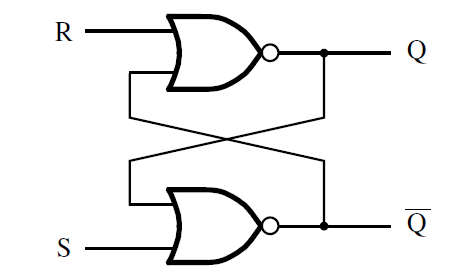
\includegraphics[width=0.4\textwidth]{Imagenes/srlatch.PNG}
	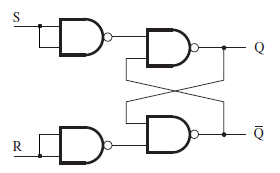
\includegraphics[width=0.4\textwidth]{Imagenes/LATCHNAND.PNG}
	\caption{Circuito Propuesto SR-Latch.}
	\label{fig:circsrlatch}
\end{figure}
Se llevará a cabo utilizando compuertas NOR y NAND, se eligió el integrado \href{https://pdf1.alldatasheet.com/datasheet-pdf/view/228632/ONSEMI/74HC02.html}{74HC02} debido a que es High-Speed y no es necesario compatibilidad con TTL, como se analizó en el punto (2). 

Se tomarán como observables  de interés el tiempo de propagación:
\begin{align} t_{p-SQ}: S \implies Q \ \ \ \textsuperscript{$\wedge$} \ \ \ t_{p-RQ}: R \implies Q \end{align} 

Estos tiempos serán comparados con un integrado \href{http://noel.feld.cvut.cz/hw/st/1937.pdf}{74HC279} el cual contiene 4 SR-Latch.

Las mediciones hechas se ven en la siguiente tabla:
\begin{table}[H]
\centering
\begin{tabular}{cccl}
\textit{}           & \textbf{Circuito NOR} & \textbf{Circuito NAND} & \textbf{74HC279} \\ \hline
\textbf{$t_{p-RQ}$} & 8.3nS                 & 43.2ns                 & 8nS              \\
\textbf{$t_{t-RQ}$} & 4.83nS                & 4nS                    & 14nS             \\
\textbf{$t_{p-SQ}$} & 24.24nS               & 18ns                   & 15nS             \\
\textbf{$t_{t-SQ}$} & 11nS                  & 4ns                    & 8nS             
\end{tabular}
\end{table}
Es notable que los tiempos son bastante similares, el espacio que ocupan no lo es, dado que toma el doble de integrados para la misma cantidad de Latches. 
\subsection{Flip Flop D}
Un Flip Flop D es un elemento de memoria sincrónico,cuenta con  2 entradas siendo una de clock y la otra de la información (Data).Le corresponde la siguiente tabla de verdad:
% Please add the following required packages to your document preamble:
% \usepackage[table,xcdraw]{xcolor}
% If you use beamer only pass "xcolor=table" option, i.e. \documentclass[xcolor=table]{beamer}
\begin{table}[H]
\centering
\begin{tabular}{
>{\columncolor[HTML]{FFFFFF}}c 
>{\columncolor[HTML]{FFFFFF}}c |
>{\columncolor[HTML]{FFFFFF}}c }
\textbf{Clock} & \textbf{$D$} & \textbf{$Q_n$} \\ \hline
$\downarrow$   & X            & $Q_{n-1}$      \\
$\uparrow$     & 0            & 0              \\
$\uparrow$     & 1            & 1             
\end{tabular}
\end{table}
El circuito propuesto de implementación es el siguiente:\footnote{Brown, S. and Vranesic, Z. (2002). Fundamentals of digital logic with VHDL design. 3rd ed. pp.254-256.}:
\begin{figure}[H]	
	\centering
	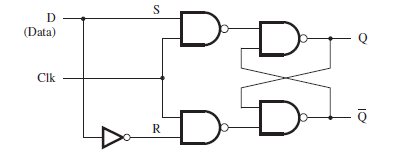
\includegraphics[width=0.8\textwidth]{Imagenes/dff.PNG}
	\caption{Circuito Propuesto Flip Flop D.}
	\label{fig:circsrlatch}
\end{figure}
Se llevará a cabo utilizando compuertas NAND, se eligió el integrado \href{https://pdf1.alldatasheet.com/datasheet-pdf/view/351460/ONSEMI/74HC132.html}{74HC132}  debido a que es High-Speed y no es necesario compatibilidad con TTL, como se analizó en el punto (2). 
También para el clock se realizó un edge-Detector implementado con el siguiente circuito:
\begin{figure}[H]	
	\centering
	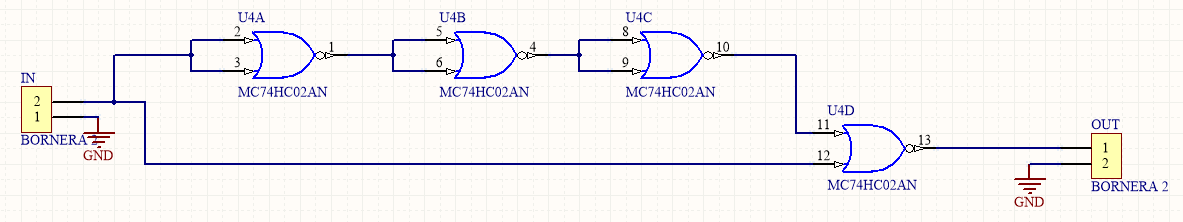
\includegraphics[width=0.8\textwidth]{Imagenes/edgedetector.PNG}
	\caption{Edge detector.}
	\label{fig:circedge}
\end{figure}
El cual es anexado al circuito implementado con NANDS del latch SR.


Se tomarán como observables  de interés el tiempo de propagación y de transición:
\begin{align} t_{p-DQ}: D \implies Q \ \ \ t_{t-DQ}: Q=0 \implies Q = 1 \end{align} 
En cuanto a la medición de estos tiempos, se tuvo la problemática de que el rise time de las compuertas eran menores que el rise time del osciloscopio, en algunas de ellas se logró conseguir un osciloscopio con mayor ancho de banda lo cual mejoró las mediciones.

Estos tiempos medidos serán comparados con un integrado \href{https://pdf1.alldatasheet.com/datasheet-pdf/view/15593/PHILIPS/74HC374.html}{74HC374} el cual contiene 8 Flip Flop D.
Las mediciones hechas se ven en la siguiente tabla:
\begin{table}[H]
\centering
\begin{tabular}{ccc}
\textit{}                               & \textbf{Circuito}         & \textbf{74HC374}     \\ \hline
\textbf{$t_{p-DQ}$}                     & 23.6nS                    & 16nS                 \\
\textbf{$t_{t-DQ}$}                     & 4.43nS                    & 5nS                  \\
\end{tabular}
\end{table}

